\documentclass[tikz,border=2pt]{standalone}
\usepackage{tikz,amsmath}
\usetikzlibrary{arrows.meta, bending,calc,decorations.markings}
\newcommand{\bmR}{\boldsymbol{\mathcal{R}}}
\begin{document}
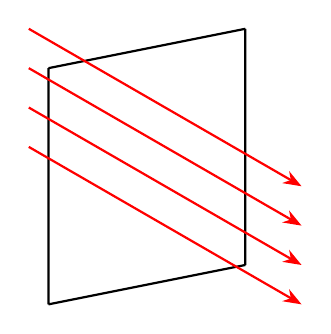
\begin{tikzpicture}[>=Stealth]

 \draw [thick] (0.5,-1.5) -- (0.5,1.5)
(3,-1) -- (3,2)
(0.5,-1.5)--(3,-1)
(0.5,1.5)--(3,2);

\foreach \y in {0, 0.5, 1.0, 1.5} {
        % Start at (0, \y), then move 4 units at a 30-degree angle
        \draw [thick, red,->] (0.25, 0.5+\y) -- ++(-30:4);
    }




\end{tikzpicture}
\end{document}